\documentclass[10pt, aspectratio=169]{beamer}
\usepackage{caption}
\usepackage{subcaption}
\usetheme[progressbar=frametitle]{metropolis}
\usepackage{amsmath}
\usepackage{siunitx}
\usepackage{xcolor}
\usecolortheme{crane}
\definecolor{craneorange}{rgb}{0.53,0.66,0.42}
\usecolortheme{spruce}
\usepackage{hyperref}
\usepackage{multimedia}
\usepackage[percent]{overpic}
\usepackage[para]{footmisc}

\title{Computational study of far-field acoustic emission by collapsing bubbles}
\date{\today}
\author[shortname]{Ratnesh K. Shukla}
\institute[shortinst]{Indian Institute of Science, Bangalore}

\begin{document}
\begin{frame}
	\maketitle
\end{frame}

\begin{frame}{Kirchhoff integral formulation}
	\begin{figure}
		\centering
		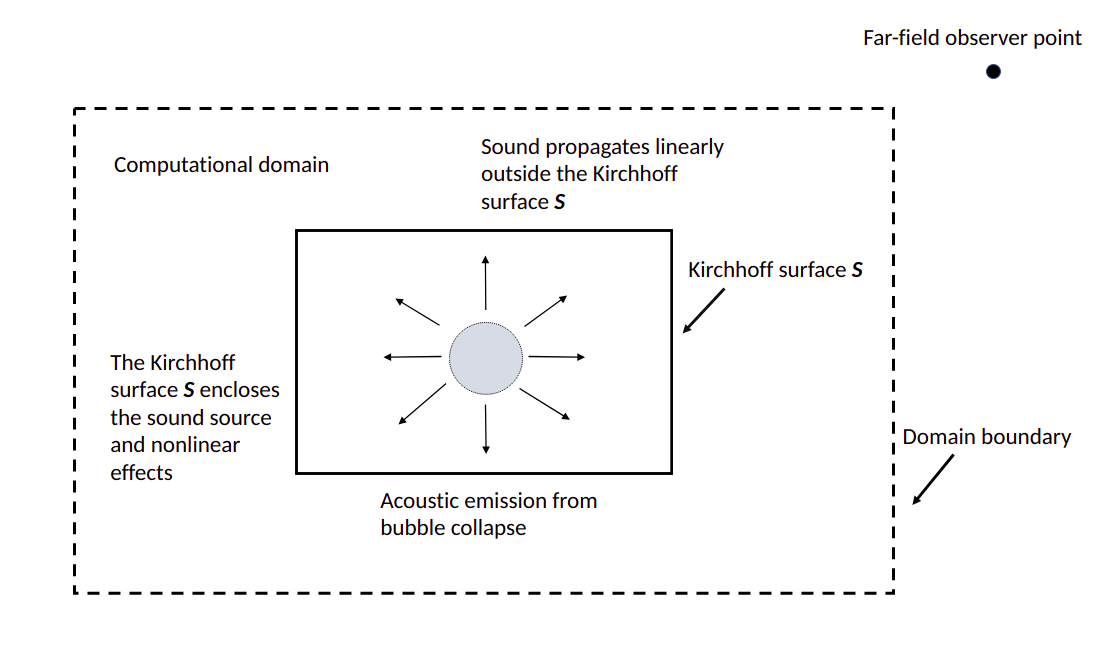
\includegraphics[scale=0.23]{images/shematic.png}
		\caption{Schematic of far-field acoustic data computed from CFD solver using the Kirchhoff integral method.}
	\end{figure}
\end{frame}

\begin{frame}{Kirchhoff integral formulation}
	\begin{itemize}
		\item Given a stationary control surface \textbf{S} that encloses the sound sources and nonlinear fluid flow effects, then the far-field acoustic pressure is computed from the Kirchhoff integral 
		\begin{equation}
			\begin{split}
				p'(\mathbf{x}, t) = -\frac{1}{4\pi}\int_{S}\Big[  \frac{p'}{r^{2}}\frac{\partial r}{\partial n} - \frac{1}{r}\frac{\partial p'}{\partial n} + \frac{1}{c r}\frac{\partial r}{\partial n}\frac{\partial p'}{\partial \tau} \Big]_{\tau} dS.
			\end{split} 
		\end{equation}
		$p'$ is the acoustic pressure satisfying the wave equation outside the control surface \textbf{S}, $c$ is the speed of sound at ambient conditions and $n$ is the normal.
		The integrands are evaluated at the emission time $\tau = t - \mathbf{r}/c$ and $\mathbf{r}= |\mathbf{x} - \mathbf{y}|$ is the distance between observer and source.
		\item The $p'$, ${\partial p'}/{\partial t}$ and ${\partial p'}/{\partial n}$ are computed from flow solver.
	\end{itemize}
\end{frame}

\begin{frame}{Validation of Kirchhoff solver - Acoustic monopole}
	\begin{itemize}
		\item We solve the acoustic wave equation
		\begin{equation}
			\Bigg( \frac{1}{c_{0}^2}\frac{\partial{}^{2}}{\partial{t}^{2}}- \nabla{}^{2} \Bigg) p'(\mathbf{x}, t)  = -q(t)\delta(\mathbf{x}), 
		\end{equation}
		for a monopole source using the \textbf{Kirchhoff} method.
		\item And compare it with the exact solution $p'(\mathbf{x}, t) = -\frac{1}{4\pi} \frac{  q(t - \frac{r}{c_{0}}) }{r}$.
		\item We chose a monopole source
		\begin{equation}
			q(t) = 2(t - t0)f_{0}^{2}\exp( -f_{0}^2(t - t_{0})^{2}), 
		\end{equation}
		where $f_{0} = 100$ is the dominant frequency and $t_{0} = \frac{4}{f_{0}}$.
	\end{itemize}
\end{frame}

\begin{frame}{Validation of Kirchhoff solver - Acoustic monopole}
	\begin{itemize}
		\item We discretize a cuboidal domain of size $[-5.0,5.0]\times[-5.0,5.0]\times[-5.0,5.0]$ using $200 \times 200 \times 200$ cells.
		\item We enclose the monopole source using a cuboidal Kirchhoff surface whose diagonally opposite points are $p_{1} = (-1.0, -1.0, -1.0)$
		and $p_{2} = (1.0, 1.0, 1.0)$.
		\item The Kirchhoff surface is discretized into square cells of size $h = 0.1$.
		\item We store the analytical pressure at cell centers and interpolate it to the Kirchhoff surface using the fourth-order WENO polynomial.
		\item We interpolate the pressure data at emission time using the Linear polynomial.
		\item The Kirchhoff Integral is computed using the two-point Gauss quadrature formula.
	\end{itemize}
\end{frame}

\begin{frame}{Validation of Kirchhoff solver - Acoustic monopole}
	\begin{figure}
		\centering
		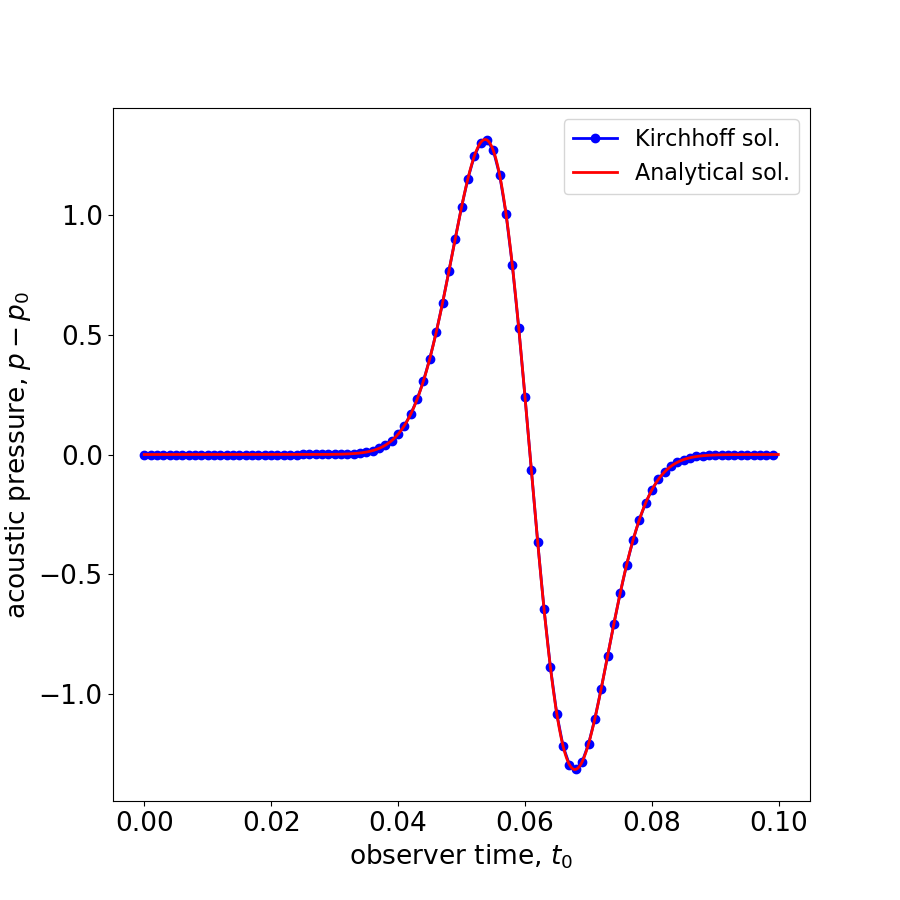
\includegraphics[scale=0.26]{images/monopole.png}
		\caption{Acoustic pressure is computed at observer point $x_{0} = (3, 3, 3)$ using the Kirchhoff method and compared with the analytical solution.}
	\end{figure}
\end{frame}

\begin{frame}{Validation of Kirchhoff solver - Euler equation}
	\begin{itemize}
		\item We solve the compressible Euler equation
		\begin{align}
			\frac{\partial \rho}{\partial t} + \nabla . (\rho \mathbf{u}) = 0,\\
			\frac{\partial \rho \mathbf{u}}{\partial t} + \nabla . (\rho \mathbf{u} \mathbf{u}) + \nabla P	 = 0,\\
			\frac{\partial E}{\partial t} + \nabla . ((E + P) \mathbf{u}) = 0,\\
			p = (\gamma - 1)(E - \frac{1}{2}\rho \mathbf{u}^{2}).
		\end{align}
		\item  for an initial density and pressure perturbation from the ambient state
		\begin{align*}
			\rho &= \rho_{0} + \rho',\\
			\mathbf{u}    &= 0,\\
			p    &= p_{0} + c_{0}^{2}\rho'. 
		\end{align*}
	\end{itemize}
\end{frame}
\begin{frame}{Validation of Kirchhoff solver - Euler equation}
	\begin{figure}
		\centering
		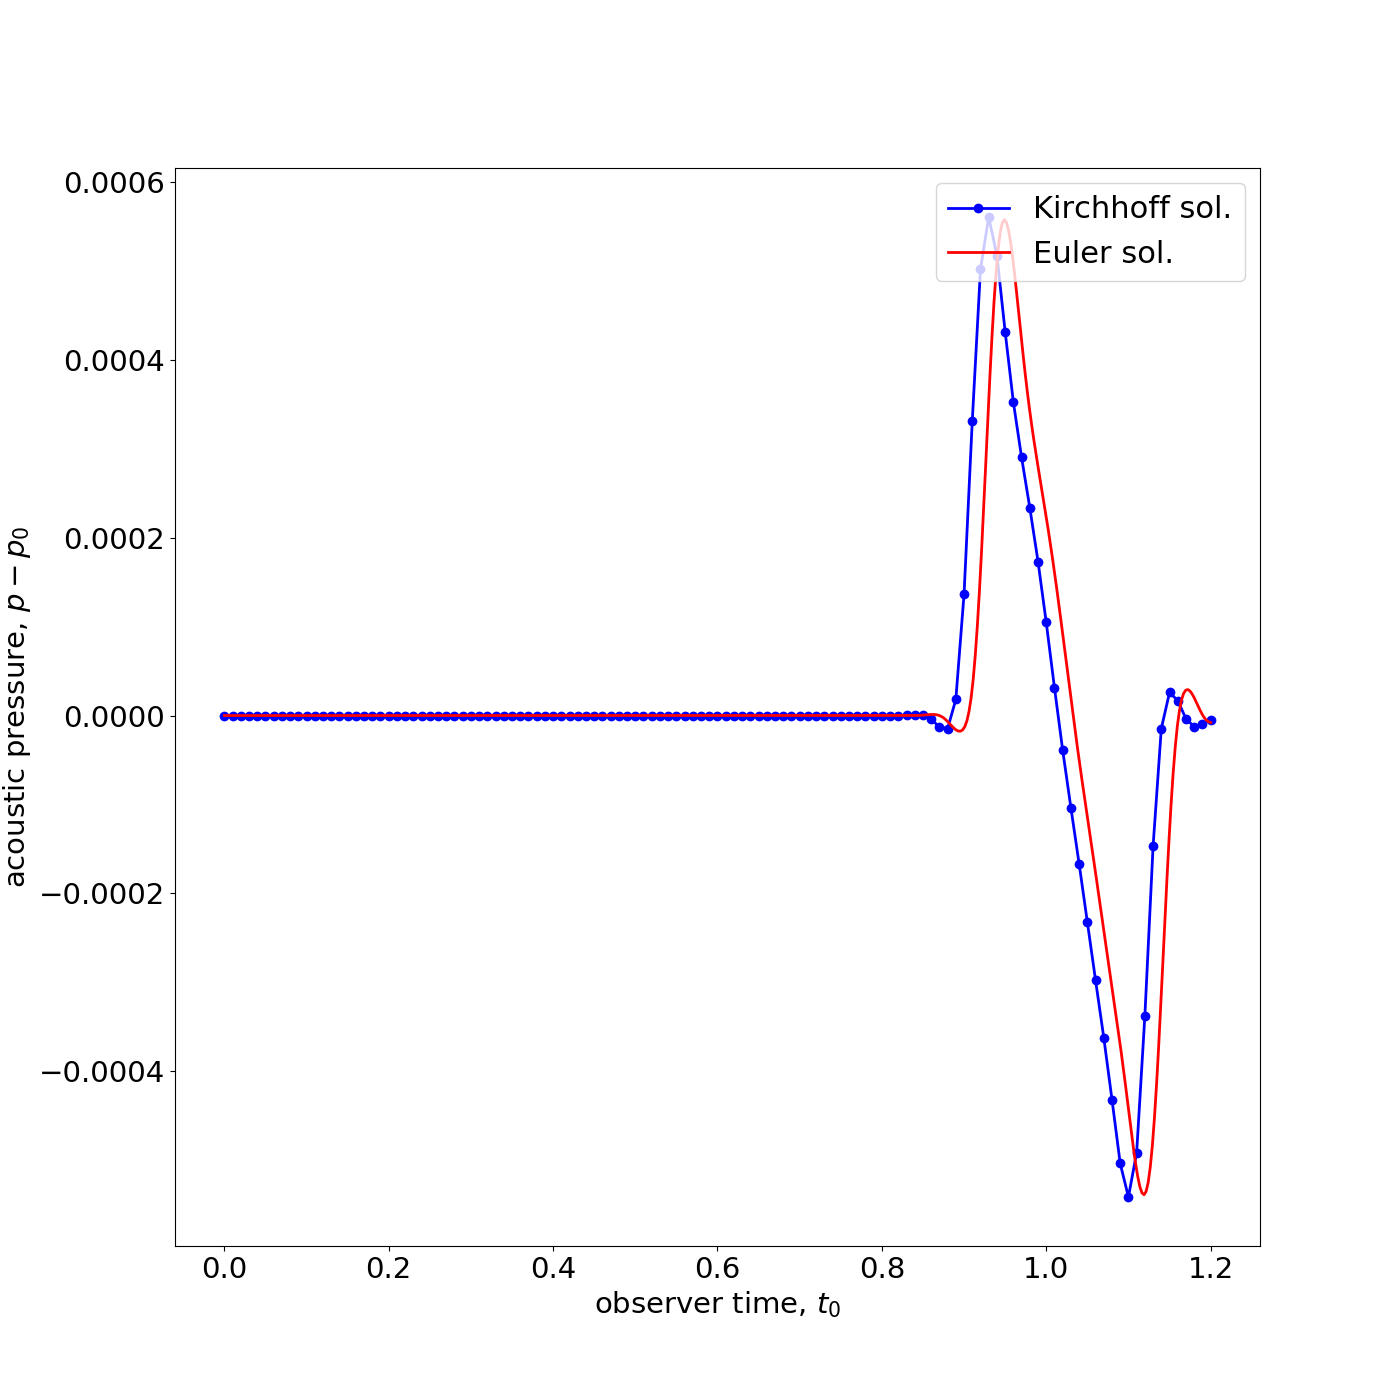
\includegraphics[scale=0.17]{images/euler.png}
		\caption{Acoustic pressure is computed at observer point $x_{0} = (0.8975, 0.8795, 0.8795)$ using the Kirchhoff method and compared with the Euler equation solution.}
	\end{figure}
\end{frame}


\begin{frame}{Acoustic emission from Rayleigh collapse of a bubble}
	
\end{frame}




\begin{frame}[standout]
	Thank you!
\end{frame}
\end{document}